\chapter{引言}\label{chap:introduction}
20世纪量子力学的一大成就是能带理论的发展,这为描述材料的电子结构提供了一种有效的语言。根据能带理论,绝缘体是导带和价带之间存在带隙的一类材料,金属则是无能隙的一类材料。绝缘体占据态全部占满,由于存在很大的能隙,加电场电子不能从价带跃迁至导带而不能导电。金属则由于能带部分占据,价带和导带直接相连,电子可以从价带移动至导带而形成电流。半导体则是介于金属和绝缘体之间,带隙比较小的一类材料。因为带隙较小,价带的部分电子也可以跃迁至导带,因而半导体有一定的导电性。在不关闭能隙的情况下,如果一个体系的哈密顿量可以绝热变换到另一个体系,我们就称这两个体系是“拓扑”等价的。我们所熟知的传统绝缘体则都是拓扑等价的,根据狄拉克理论,他们又都等价于真空。但是并不是所有的绝缘体都等价于真空。有一类绝缘体体态绝缘,但是表面导电,这类绝缘体在不关闭带隙的情况下则不能通过绝热变换变为传统的绝缘体或者真空态,称之为拓扑绝缘体。从传统绝缘体到拓扑绝缘体的相变过程并不伴随着对称性的破缺,因此不能用朗道相变理论来解释。
从体态能带色散上看,也并不能直接看出拓扑绝缘体和传统绝缘体的本质区别来,这说明二者的区别不体现在体能带的色散上。在应用方面,拓扑绝缘体表面的导电模式相比普通金属的导电模式而言有天然的优势,对杂质、形变等非磁性扰动非常稳定。另一方面,科学家还发现拓扑绝缘体有望在实现拓扑超导方面、量子计算机、信息传输等诸多方面发挥重要作用。考虑到这些潜在的价值,拓扑态的研究吸引了一大批凝聚态物理学家投身其中探索究竟。那么怎么区分普通的绝缘体和拓扑绝缘体呢?怎么寻找可能的拓扑材料呢?

随着量子霍尔效应,量子反常霍尔效应,量子自旋霍尔效应的发现,科学家们对这个问题的理解一步步深入。回答这个问题就需要拓扑能带理论,即必须要通过波函数的性质来理解,这正是最早科学家们只关注能带色散而忽略的地方。随着对这些问题的理解,科学家们又发现了一些新奇的拓扑物态,包括拓扑晶体绝缘体,拓扑半金属。只有充分了解这些物态的本质,才可能寻找越来越多有趣实用的材料,为实验和工业的应用方面提供动力,进一步推动材料科学的发展。
在本章中,我们将回顾这段历史的发展,拨云见日,逐渐理解这些新兴的量子物态,最终达到有能力寻找更多新奇拓扑材料的目的。


\section{霍尔效应}
我们的故事首先要从霍尔效应(HE)讲起。美国物理学家霍尔(Edwin H. Hall)在1879年发现\citep{hall1879},当将承载纵向电流的导体放置在垂直磁场中时,载流子将横向偏转,从而导致横向的电压,如图~\ref{fig:1-1}(a)。霍尔系数即定义为 $R_0=\frac{E_y}{I_x H}=\frac{\rho}{H}$,在自由电子近似下又满足$R_0=-\frac{1}{ne}$。
由经典电磁学知识,我们知道载流子之所以在磁场中发生偏转是因为受到洛伦兹力的作用。霍尔效应在凝聚态理论中有着非同寻常的“王者”地位,利用它可以识别载流子类型,测量载流子密度或磁场的强度。很快两年后,在1881年~\citep{hall1881},霍尔又在铁磁性材料中发现其压电效应是非磁性导体的十倍,这种更强的效应不需要外加磁场就能实现,因而被称作反常霍尔效应(Anomalous Hall effect,简称AHE),如图~\ref{fig:1-1}(c)。经过在铁,钴,镍这类铁磁材料的实验研究基础上,科学家们\citep{Pugh1930,Pugh1932}提出了反常霍尔电阻的经验公式:
\begin{equation}
    \label{eq:1-1}
    \rho_{x y}=R_{0} H_{z}+R_{s} M_{z}
\end{equation}
第一项$R_0$已经可以理解,只依赖载流子密度。但是第二项则跟材料具体情况有关,是由瞬时磁场导致的反常霍尔电阻项。这一项的存在正说明了,即使外磁场$H=0$,即没有洛伦兹力,仍然存在某种霍尔效应。早在1954年,Karplus和Luttinger \citep{karplus54}对反常霍尔效应这个问题提出一个理论解释,他们发现对于铁磁导体所有占据态的反常速度之和是非零的,所以导致霍尔电导$\sigma_{xy}$非零。又因为这个贡献只与能带结构有关,而与散射无关,因而称之为本征(或内秉)的反常霍尔效应。他们认为这个机制导致反常霍尔电阻正比于横向电阻的平方:$\rho_{x y} \propto \rho_{x x}^{2}$。除此之外,还有两个外秉的贡献也被认为是引起反常霍尔效应的主导机制。一个是Smit提出来的螺旋散射(skew scattering)\citep{SMIT1955877,SMIT195839},认为真实材料中总是存在反对称的杂质散射,从而导致电子的横向运动,并且这个机制导致的反常霍尔电阻正比于横向电阻:$\rho_{x y} \propto \rho_{x x}$。另一个是Berger在1970年提出来的边跳机制(side jump)~\citep{Berger1970},认为AH电流的主要来源是准粒子在自旋轨道耦合(spin-orbit coupling, 简称SOC)杂质的散射下经历的侧跳。令人惊奇的是,这种半经典的预测竟然发现AHE对于杂质密度和强度的依赖都没有,所以得到了与内秉机制相同的反常霍尔电阻依赖关系:$\rho_{x y} \propto \rho_{x x}^{2}$。

反常霍尔速度这一项事实上是非常复杂的,并不仅仅比例于$M_z$。直到贝利(Berry)在1984年提出贝利相位(Berry phase)这一拓扑和几何的概念之后~\citep{Berry1802},反常霍尔效应才被人们所理解。简单来讲,这一反常霍尔速度来源于占据态波函数的贝利曲率(Berry curvature),而它充当了动量空间“磁场”的作用~\citep{MacDonald}。

\begin{figure}[!htbp]
    \centering
    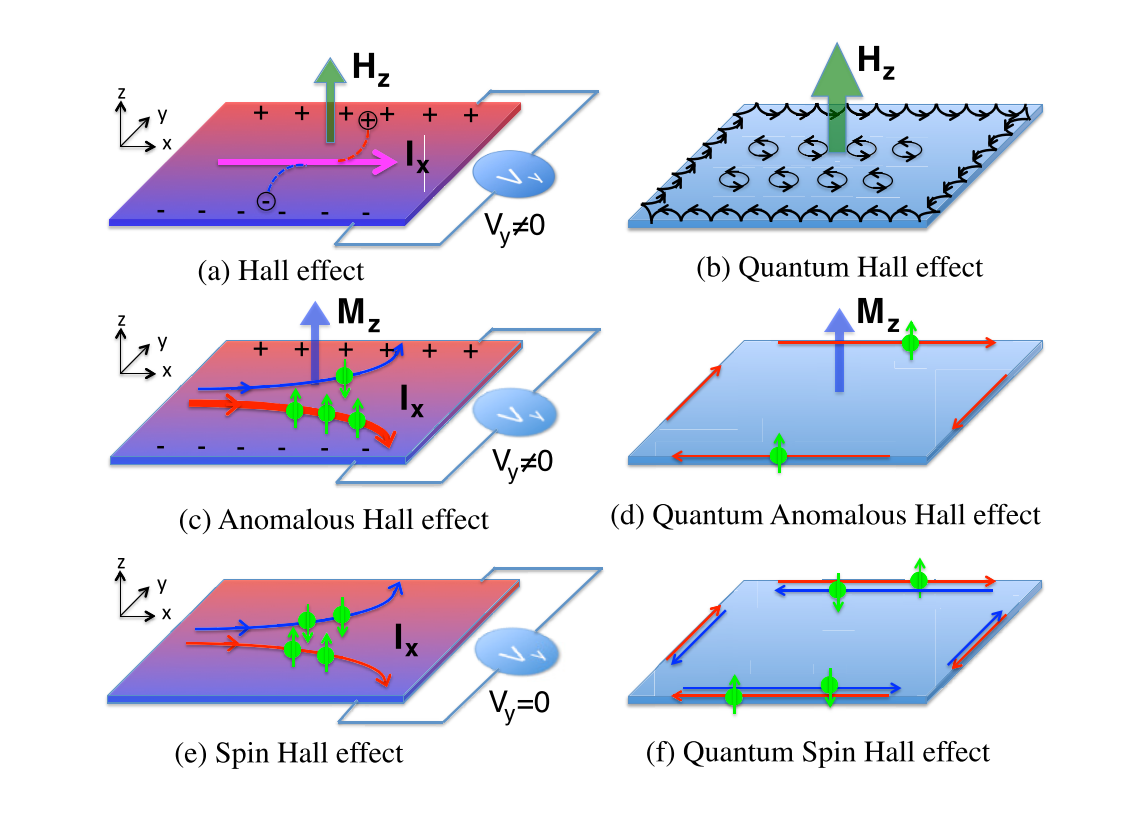
\includegraphics[width=10 cm]{chapter1-1.png}
    \bicaption{(a)霍尔效应。(b)量子霍尔效应。(c)反常霍尔效应。(d)量子反常霍尔效应。(e)自旋霍尔效应。(f)量子自旋霍尔效应。(图片来自\citep{review-arxiv})}
    {(a) Hall effect.  (b) Quantum Hall effect. (c) Anomalous Hall effect. (d) Quantum Anomalous Hall effect.  (e) Spin Hall effect. (f) Quantum Spin Hall effect. (From \cite{review-arxiv})}
    \label{fig:1-1}
\end{figure}

\section{量子霍尔效应}
1980年,Klaus von Klitzing 发现~\citep{Klitzing1980},在非常低的温度下,霍尔电导作为垂直于二维(2D)电子气平面施加的磁场强度的函数,会出现量化的阶梯平台,同时纵向电导为零。这就是著名的量子霍尔效应 (Quantum Hall effect, 简称QHE) 。在量子霍尔效应中,如果对二维体系加一个外磁场$H_z$,电子的回旋运动将形成朗道能级。磁场足够强时,体内的电子将局域在体内做圆周运动,但在边界上因为无法做圆周运动而形成沿着特定方向的边缘运动,如图~\ref{fig:1-1}(b)。而且这些边缘态不会受到杂质的影响。因而载流子的运动是无耗散的,霍尔电导被量化为以$e/h$为单位的量子数$n$,且该量子数$n$与边缘态的数量相对应。后来研究发现,无论是整数还是分数的量子霍尔效应都可以由电子波函数的拓扑性质来解释\citep{Laughlin1981,TKNN1982}。从久保公式得出的霍尔电导里的整数,最初称为TKNN数,其实就是现在被用于表征拓扑不变性的“陈数”(Chern number)。后来,我们把具有非零陈数的二维材料,称为陈绝缘体。所以,陈绝缘体的拓扑分类是$\mathbb{Z}$分类。
\begin{figure}[!htbp]
    \centering
    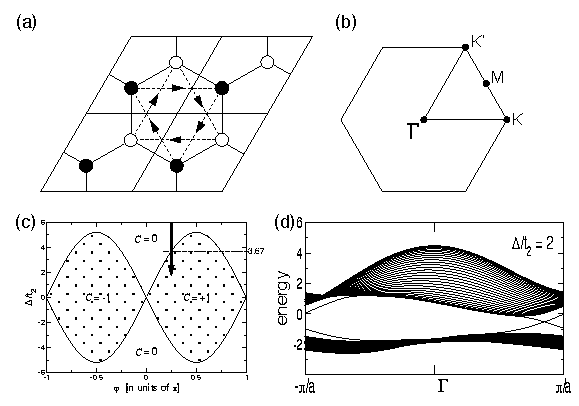
\includegraphics[width=8.5cm]{chapter1-2.pdf}
    \bicaption{(a)Haldane模型的四个原胞。(b)Haldane模型的第一布里渊区。(c)Haldane模型的Chern数,作为参数 $\varphi$ 和 $\Delta/ t_2$ ($t_1=1, t_2=1/3$)的函数。(d)$b_2$方向无限长,而$b_3$方向包含30个原胞的带状格子的能量随波矢$k_y$的变化,$\Delta/t_2 <(\Delta/t_2)_{cr}$。 可以看到手性边界态。(图片来自\citep{Haldane2})}
    {(a) Four unit cells of the Haldane model. (b) First Brillouin zone of the Haldane model. (c) Chern number of the bottom band of the Haldane model as a function of the parameters $\varphi$ and $\Delta/ t_2$ ($t_1=1, t_2=1/3$). (d) Energy vs wave vector $k_y$ for the Haldane model in a
    strip geometry 30 cells wide along the $b_3$ direction and extending infinitely along $b_2$ direction,$\Delta/t_2 <(\Delta/t_2)_{cr}$. Chiral edge states are visible. ( From \cite{Haldane2})}
    \label{fig:1-2}
\end{figure}

第一个超越量子霍尔效应的一个简单的例子是由Haldane在1988年提出的在周期磁场中的石墨烯模型,后称之为Haldane模型\citep{haldane1988model,Haldane2}:
\begin{equation}
    \label{eq:1-2}
    \begin{split}
    \mathbf{H}(\mathbf{k})=&2 t_{2} \cos \phi\left(\sum_{i} \cos \left(\mathbf{k} \cdot \mathbf{b}_{i}\right)\right) \mathbf{I}+t_{1}\left(\sum_{i}\left[\cos \left(\mathbf{k} \cdot \mathbf{a}_{i}\right) \sigma^{1}+\sin \left(\mathbf{k} \cdot \mathbf{a}_{i}\right) \sigma^{2}\right]\right)\\
    &+\left[\Delta-2 t_{2} \sin \phi\left(\sum_{i} \sin \left(\mathbf{k} \cdot \mathbf{b}_{i}\right)\right)\right] \sigma^{3}
    \end{split}
\end{equation}
这个模型如图~\ref{fig:1-2}(a,b),是在二维石墨烯模型的基础上,引入复数的次近邻跃迁(hopping)。$t_{1}$是最近邻不同子格之间的hopping。$t_{2} e^{\pm i \varphi}$就是复数的次近邻hopping(相同子格子之间的hopping)。这个复数hopping的引入使得二维平面有一个周期的磁通,但是体系总磁通仍然为零,这打破了体系原有的时间反演对称性。并且由于A,B子格子的占位能不同(分别为$\Delta,-\Delta$),所以体系不再保持空间反演对称性。
这样一个模型就可以通过改变参数$\varphi, t_2, \Delta$研究普通绝缘体到陈绝缘体的相变\citep{haldane1988model,Haldane2},如图~\ref{fig:1-2} (c) 。当调节参数使得体系进入陈数非零的相时,计算$b_3$方向包含30个原胞的有限厚度的哈密顿量的能带结构,如图~\ref{fig:1-2} (d) ,确实可以在带隙中看到存在两条导电的手性边界态,分别来自左右两个边界。Haldane模型是超越量子霍尔效应之外的拓扑绝缘体的第一个例子。与量子霍尔效应不同的是Haldane模型磁通整体其实是0,也就是说并不需要外加一个磁场就可以实现非平庸的拓扑,即量子反常霍尔效应 (Quantum Anomalous Hall effect, 简称QAHE),如图~\ref{fig:1-1} (d) 。通常把类似于Haldane模型所描述的破坏时间反演对称性且具有非平庸陈数的系统称为陈绝缘体。但是因为这个模型需要手动加入磁通,因而无法在真实材料中实现。
%The Quantum Anomalous Hall Effect has recently been observed in thin films of chromium-doped (Bi,Sb)2Te3 [8].【short review】

\begin{figure}[!t]
    \centering
    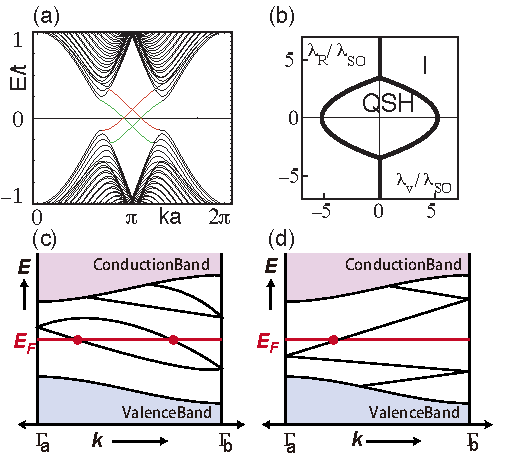
\includegraphics[width=8cm]{chapter1-3.pdf}
    \bicaption{(a)QSH相的一维锯齿形边界能谱。(b)相图,作为以$\lambda_v$ 和 $\lambda_R$ 为变量的函数,$0 < \lambda_{\mathrm{SO}} \ll t$。(c,d)在两个边界克拉默简并点$\Gamma_a=0$和$\Gamma_b=\pi/a$之间的电子色散。在(c)中,表面态穿过费米能$E_F$偶数次,在(d)中,表面态穿过费米能$E_F$奇数次。穿过奇数次的表面态是受拓扑保护的金属边界态。(图片来自\citep{kane2,TIreview,Fu2007topo})}
    { Energy bands for a one-dimensional ‘‘zigzag’’ strip in the (a) QSH phase $\lambda_v=0.1 t$, $\lambda_{SO}=0.06 t$, $\lambda_{R}=0.05 t$. The edge states on a given edge cross at $ka=\pi$. (b)The phase diagram as a function of $\lambda_v$ and $\lambda_R$ for $0 < \lambda_{\mathrm{SO}} \ll t$. (c,d) Electronic dispersion between two boundary Kramers degenerate points $\Gamma_a=0$ and $\Gamma_b=\pi/a$.In (c) the number of surface states crossing the Fermi energy $E_F$ is even, whereas in (d) it is odd. An odd number of crossings leads to topologically protected metallic boundary states. (From~\citep{kane2,TIreview,Fu2007topo})}
    \label{fig:1-3}
\end{figure}

当存在时间反演对称性时,体系的霍尔电导总是为零。那么很自然的就会产生疑问,时间反演对称性是否可以保护非平庸的拓扑呢?换句话说,是否存在时间反演不变的拓扑绝缘体呢?答案是肯定的。那么首先对方程\ref{eq:1-2}做傅立叶变换,Haldane模型在实空间可以写作:
% \begin{equation}
%     \label{eq:1-3}
%     H=t_{1} \sum_{\langle i, j\rangle} c_{i}^{\dagger} c_{j}+t_{2} \sum_{\langle\langle i, j\rangle\rangle} e^{-i \varphi \nu_{ij}} c_{i}^{\dagger} c_{j}+\Delta \sum_{i \in A} c_{i}^{\dagger} c_{i}-\Delta \sum_{i \in B} c_{i}^{\dagger} c_{i}
% \end{equation}

\begin{equation}
    \label{eq:1-3}
    H=t_{1} \sum_{\langle i, j\rangle} c_{i}^{\dagger} c_{j}+t_{2} \sum_{\langle\langle i, j\rangle\rangle} e^{-i \varphi \nu_{ij}} c_{i}^{\dagger} c_{j}+\Delta \sum_{i}\xi_{i} c_{i}^{\dagger} c_{i}
\end{equation}
这里次近邻复数的hopping  $t_2 e^{i\varphi \nu_{ij} }$是由于施加磁场带来的,其中$\nu_{ij}=-\nu_{ji}=\pm 1$取决于最近邻成键的方向。Kane和Mele在Haldane模型的基础上加以修改,认为次近邻之间复数的hopping来自自旋轨道耦合作用\citep{Kane2005,kane2}。Kane-Mele模型可以看作是两个Haldane模型的时间反演版本:
% \begin{equation}
%     \label{eq:1-4}
%     \begin{aligned}
%     H &=t \sum_{\langle i, j\rangle s} c_{i s}^{\dagger} c_{j s}+i \lambda_{\mathrm{so}} \sum_{\langle\langle i, j\rangle\rangle s s^{\prime}} \nu_{i j} c_{i s}^{\dagger} \sigma_{s, s^{\prime}} c_{j s^{\prime}}+i \lambda_{R} \sum_{\langle i, j\rangle s s^{\prime}} c_{i s}^{\dagger}\left(\boldsymbol{\sigma} \times \mathbf{d}_{i j}\right)_{s s^{\prime}}^{z} c_{j s^{\prime}}^{\dagger} \\
%     &+\lambda_{v} \sum_{i \in A, s} c_{i s}^{\dagger} c_{i s}-\lambda_{v} \sum_{i \in B, s} c_{i s}^{\dagger} c_{i s}
%     \end{aligned}
% \end{equation}
\begin{equation}
    \label{eq:1-4}
    \begin{aligned}
    H=& t \sum_{\langle i j\rangle} c_{i}^{\dagger} c_{j}+i \lambda_{\mathrm{SO}} \sum_{\langle\langle i j\rangle\rangle} \nu_{i j} c_{i}^{\dagger} s^{z} c_{j}+i \lambda_{R} \sum_{\langle i j\rangle} c_{i}^{\dagger}\left(\mathbf{s} \times \hat{\mathbf{d}}_{i j}\right)_{z} c_{j}+\lambda_{v} \sum_{i} \xi_{i} c_{i}^{\dagger} c_{i}
    \end{aligned}
\end{equation}
其中$t$相当于$t_1$,$\lambda_{\mathrm{SO}}$相当于$t_2$,是自旋轨道耦合带来的复数hopping。因为每个格点有自旋上、自旋下两个轨道,所以体系仍然有时间反演对称性。$\lambda_{v}$相当于$\Delta$,使得两个子格子占位能占位能不同。$\lambda_{R}= 0$时,自旋上下没有耦合。但是实际体系中往往满足$\lambda_{R}\neq 0$,此时则破坏镜面对称性$M_z$,使得自旋上下的电子之间发生杂化,自旋不再是好的量子数。但是计算发现,此时仍然可以具有拓扑保护的边界态,边界态的数目模2仍然是拓扑不变量,所以其拓扑分类是$\mathbb{Z}_2$分类的\citep{kane2}。这就是我们熟知的QSHE,也称为$\mathbb{Z}_2$拓扑绝缘体,如图~\ref{fig:1-1}(f)。不像量子霍尔效应和量子反常霍尔效应那样,量子自旋霍尔效应的边界导电通道是自旋分辨的,即每个通道只能有一种自旋的电子通过。关于量子自旋霍尔效应的的边缘态是否有很好的弹道输运性质仍然有些争议,但是最近发表在《自然物理》杂志上的一篇文章中,作者证明了由时间反演等反幺正算符保护的边界态是很容易与环境发生耦合的,因而是不稳定的~\citep{2020Fragility},这让我们对这个问题有了一个新的认识。

\section{拓扑绝缘体}\label{sec:system}
在前面的小节,我们已经简单介绍了霍尔效应和它的量子化版本。我们知道了在有时间反演对称性的体系中,也可以有拓扑不平庸的态,即Kane-Mele模型所描述的量子自旋霍尔效应态。然而,这个在石墨烯模型中提出来的理论模型仍然很难在实验上研究,因为在石墨烯中自旋轨道耦合作用非常小,只有$10^{-3}$ meV。随后,斯坦福大学的张首晟等人提出的BHZ模型,预言可以在HgTe/CdTe量子阱中,通过调节量子阱的厚度来研究正常态和量子自旋霍尔态之间的相变,如图~\ref{fig:1-4}(a,b)~\citep{bernevig2004}。
%在基矢$\left|E 1, m_{I}=\frac{1}{2}\right\rangle$,$\left|H 1, m_{I}=\frac{3}{2}\right\rangle$,$\left|E 1, m_{I}=-\frac{1}{2}\right\rangle$和$\left|H 1, m_{I}=-\frac{3}{2}\right\rangle$下,
这个结构的晶格模型可以写作~\citep{bernevig2004,Asboth2015}:
\begin{equation}
    \label{eq:1-5}
    \left.\hat{H}_{\mathrm{BHZ}}(\mathbf{k})=\hat{s}_{0} \otimes\left[\left(u+\cos k_{x}+\cos k_{y}\right) \hat{\sigma}_{z}+\sin k_{y} \hat{\sigma}_{y}\right)\right]+\hat{s}_{z} \otimes \sin k_{x} \hat{\sigma}_{x}+\hat{s}_{x} \otimes \hat{C}
\end{equation}
调节合适的耦合参数C,可以使模型满足时间反演对称性,且$\mathcal{T}^2=-1$。他们发现当HgTe厚度达到临界厚度$d=d_c$时(当模型参数$u=-2$),正常态将到达一个能带反转的态,当HgTe厚度大于临界厚度$d>d_c$,体系进入量子自旋霍尔态。此时可以观察到量子化的霍尔电导。 很快这一理论就被实验所证实~\citep{konig2007quantum},并且在特定厚度的量子阱内观察到量子自旋霍尔边缘态,如图~\ref{fig:1-4}(c)。
\begin{figure}[!t]
    \centering
    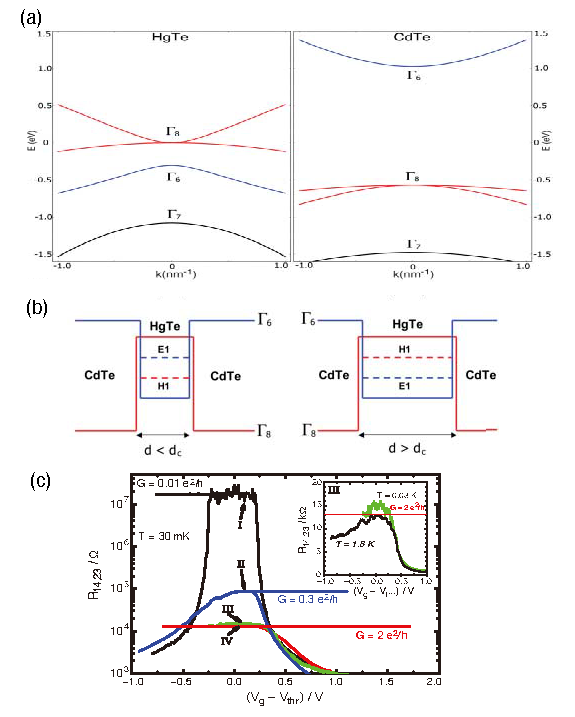
\includegraphics[width=8.5cm]{chapter1-4.pdf}
    \bicaption{(a)HgTe和CdTe在$\Gamma$点附近的体能带图。(b)CdTe-HgTe-CdTe量子阱,在$d < d_c$时E1 > H1,处于正常态。在$d > d_c$时E1 < H1,处于能带反转范围。红色代表$\Gamma_8$表示,蓝色代表$\Gamma_6$表示。(c)纵向四端电阻$R_{14,23}$在不同厚度下随着电压的变化。(图片来自\citep{bernevig2004,konig2007quantum})}
    { (a) Bulk energy bands of HgTe and CdTe near the $\Gamma$ point. (b) The CdTe-HgTe-CdTe quantum well in the normal regime E1> H1 with $d < d_c$ and in the inverted regime H1> E1 with $d > d_c$. $\Gamma_8$/H1 symmetry is indicated in red and $\Gamma_6$/E1 symmetry is indicated in blue. (c) The longitudinal four-terminal resistance, $R_{14,23}$, of various normal (d = 5.5 nm) (I) and inverted (d = 7.3 nm) (II, III, and IV) quantum well structures as a function of the gate voltage measured for B=0 T at T = 30 mK. (From~\citep{bernevig2004,konig2007quantum})}
    \label{fig:1-4}
\end{figure}
所以HgTe/CdTe量子阱是第一个在实验上实现的二维拓扑绝缘体 (Topological insulator,简称TI) 。因为HgTe天然的具有能带反转的特点,BHZ方法的特别之处是利用HgTe这一特点第一次给出了通过调节能带反转来实现非平庸的拓扑,这也为今后对拓扑材料的研究提供了新的思路。但是由于这类材料含毒性元素且热稳定性差,所以在实验制备上带了困难。在2008年, 张首晟研究组又提出一种新的二维拓扑绝缘体材料: AlSb/InAs/GaSb/AlSb 量子阱~\citep{zhang2008,InAs},这类材料也可以实现能带反转,有望在实验上有更广阔的应用。

如上一小节的讨论,时间反演对称性可以保护二维拓扑绝缘体,也称为$\mathbb{Z}_2$拓扑绝缘体。其表面导电模式只能有奇数个,偶数个的表面模式则不能被时间反演保护而打开能隙。这样的量子自旋霍尔态可以通过在二维平面上对占据态的波函数定义一个$\mathbb{Z}_2$不变量来描述。
%这个不变量的详细形式,我们会在后面的小节里仔细讨论。
时间反演保护的拓扑绝缘体还可以扩展到三维(3D)~\citep{Fu2007topo,Fu2007IS}。三维拓扑绝缘体由四个$\mathbb{Z}_2$:$v_0;(v_1,v_2,v_3)$来刻画,$v_0$是一个强拓扑指标,$(v_1,v_2,v_3)$是三个弱拓扑指标,即定义在$k_{x,y,z}=\pi$的面上的$\mathbb{Z}_2$指标。$v_0=0$代表是弱拓扑绝缘体(WTI),$v_0=1$代表强拓扑绝缘体(STI)。弱拓扑绝缘体可以看作是由二维的QSH沿某一个方向堆叠而成,有偶数个表面模但是很容易由杂质破坏,如图~\ref{fig:1-3} (c) 。强拓扑绝缘体则可以看作是由一个QSH和一个拓扑平庸的二维绝缘体交替堆叠而成,有奇数个可以导电的表面态,而且非常稳定,不受弱无序和相互作用的影响 ,如图~\ref{fig:1-3} (d) 。并且不同于二维拓扑绝缘体,三维拓扑绝缘体的表面狄拉克锥除了狄拉克点之外,自旋都是非简并的。在表面狄拉克锥的任意一点自旋动量锁定在一起(spin-momentum locking),如Bi$_2$Se$_3$~\citep{spin2013},由于时间反演和$C_{3v}$对称性,在表面狄拉克锥的任意一个固定的动量$\mathbf{k}$点,哈密顿量形如$\hat{H}=
A (\vec{k} \times \vec{\sigma})$,即自旋总是垂直于动量$\mathbf{k}$,从而
形成独特的螺旋状自旋结构,对于自旋电子学的研究带来了新的途径。

对于有中心反演对称的体系,傅亮和Kane提出了一套简单通过对称性指标就能判断拓扑绝缘体的方法~\citep{Fu2007IS}。并且利用这套方法,2008年,他们首先提出了在$\mathrm{Bi}_{1-x} \mathrm{Sb}_{x}$合金中可以通过掺杂实现三维拓扑绝缘体\citep{fuBiSe},第二年便被角分辨光电子实验所证实\citep{2009hsieh}。这是第一个理论预言并被实验确认的三维拓扑绝缘体。但是因为这个体系的缺点是带隙较小,且是合金,所以表面结构复杂而不易研究。2009年,我们组的方忠、戴希团队提出无需掺杂的层状结构Bi$_2$Se$_3$家族是体态绝缘,表面有狄拉克锥的三维拓扑绝缘体~\citep{zhang2009topological}。Bi$_2$Se$_3$是层状材料,但是层与层之间有一定的相互作用,在考虑自旋轨道耦合时,体能带发生反转且体能隙能达到0.3 eV,有非常强的抗热扰动能力。表面狄拉克点处于费米能附近,且具有非常好的线性色散。这样优质的特点为实验研究提供了非常良好的平台。同年,即被多个实验组所证实~\citep{chen2009experimental,xia2009,hsieh2009}。目前这个家族仍然是作为三维拓扑绝缘体研究最多的材料。顺便提一下,2010年,物理所方忠、戴希团队提出在Bi$_2 $Se$_3$家族中掺Cr,Fe等金属元素可以实现陈绝缘体~\citep{Yu61},随后清华大学薛其坤团队在此体系中第一次观察到量子反常霍尔效应~\citep{xue13},这是Bi$_2 $Se$_3$家族的又一次重大突破。此后,随着人们对拓扑绝缘体的认识越来越深刻,理论计算和实验的手段越来越先进,有越来越多的材料被发现是拓扑绝缘体,包括在三元化合物TlBi$X_2$和TlSb$X_2$($X$=S,Se,Te)系列~\citep{Yan2010,chen10},half-Heusler材料~\citep{half2010}和黄铜矿结构(Chalcopyrite) ~\citep{Feng2011}中发现了很多拓扑绝缘体(其中部分材料我们后来发现其实是外尔半金属,将在第五章详细讨论),还有翁红明、方忠、戴希等发现的准二维大能隙拓扑绝缘体ZrTe$_5$~\citep{wengzrte},还有层状材料ZrSiS家族在考虑自旋轨道耦合时是弱拓扑绝缘体~\citep{xu2015two}等等。

如上所述,凝聚态物理短短几年内在拓扑绝缘体上已经取得了显著的成果,这期间中国物理学者发挥了重要的作用。理论和实验方面相辅相成,结束了对于量子反常霍尔效应20多年的追寻。但是,我们不得不承认这只是在科学史上的一小步,离实际应用还有很大的距离。因为这一次观察量子反常霍尔效应还需要在 100 mK 下的极低温实验室条件里才能实现。所以想要得到应用,就必须要突破在室温下就能实现这一目标。近几年来,随着理论物理学家在磁性理论方面取得的一系列进展~\citep{Watanabe2018,Elcoro2020,xuyf2020,Peng2021},大家开始逐渐将注意力转向不需要掺杂的磁性材料领域,以期在本征的磁性材料内找到量子反常霍尔效应的候选体。
%{\color{red}{ Co3Sn2S2,MnBi2Te4 掀起了这个领域的一个热潮。本论文将在后面的小节里对这几个材料详细介绍}}
2018年,两个团队几乎同时在铁磁外尔半金属Co$_3$Sn$_2$S$_2$中发现了巨反常霍尔效应~\citep{cosns2018,2017Giant}。
相比Cr掺杂的(Bi,Sb)$_2$Te$_3$的铁磁居里温度15K而言,这个材料的居里温度可以达到175K,为高温霍尔效应的研究提供了平台。
另一个明星材料是层状材料MnBi$_2$Te$_4$,它首先被预言为本征的反铁磁拓扑绝缘体~\citep{zhanghj2019,Li2019}。随后实验上又发现奇数层的MnBi$_2$Te$_4$薄膜可以出现净磁矩,甚至可以出现反常霍尔效应~\citep{zhanghj2019,mnbite2,mnbite3,mnbite4,mnbite5}。并且实验上进一步发现在MnBi$_2$Te$_4$中插入Bi$_2$Te$_3$层形成超晶格结构MnBi$_6$Te$_{10}$或者MnBi$_8$Te$_{13}$,使层间反铁磁耦合降低,不需要外场驱动就可以实现净磁矩,从而实现真正的反常霍尔效应~\citep{tian2020,hu2020}。相信这些进展会为实现室温反常霍尔效应提供强有力的动力,也期待这一天早日到来。


\section{拓扑晶体绝缘体}\label{sec:tci}
在前面两个小节的介绍中,我们知道陈绝缘体不受任何对称性保护,其拓扑分类是$\mathbb{Z}$分类。受时间反演对称性保护的绝缘体虽然其陈数总是为零,但是却可以存在$\mathbb{Z}_2$分类,即平庸的偶数类和不平庸的奇数类两类。那么我们就会问,在$\mathbb{Z}_2$为偶数的平庸分类里,是否也存在更加细致丰富的拓扑分类呢?答案是肯定的。当考虑到晶体的对称性时,如旋转对称性,中心反演对称性,镜面对称性等,即使$\mathbb{Z}_2$平庸的一类里,仍然可以存在由其他晶体对称性保护的不平庸拓扑分类,这就是所谓的拓扑晶体绝缘体 (Topological crystalline insulator,简称TCI)。可以说,该领域的发展非常之迅速。2011年,傅亮等人第一次提出拓扑晶体绝缘体的概念~\citep{fu2011topological}。2018年方辰老师团队将第二类磁群保护的拓扑晶体绝缘体完全分类~\citep{song2017}。2021年,方辰老师团队又利用“实空间方法”(real-space recipe)对其他三类磁群对称性保护的拓扑晶体绝缘体做了完整分类~\citep{Peng2021}。从拓扑晶体绝缘体的提出到完全分类只用了10年的时间。在本小节中将根据时间顺序简单梳理一下拓扑晶体绝缘体的发展历史。

\begin{figure}[!htbp]
    \centering
    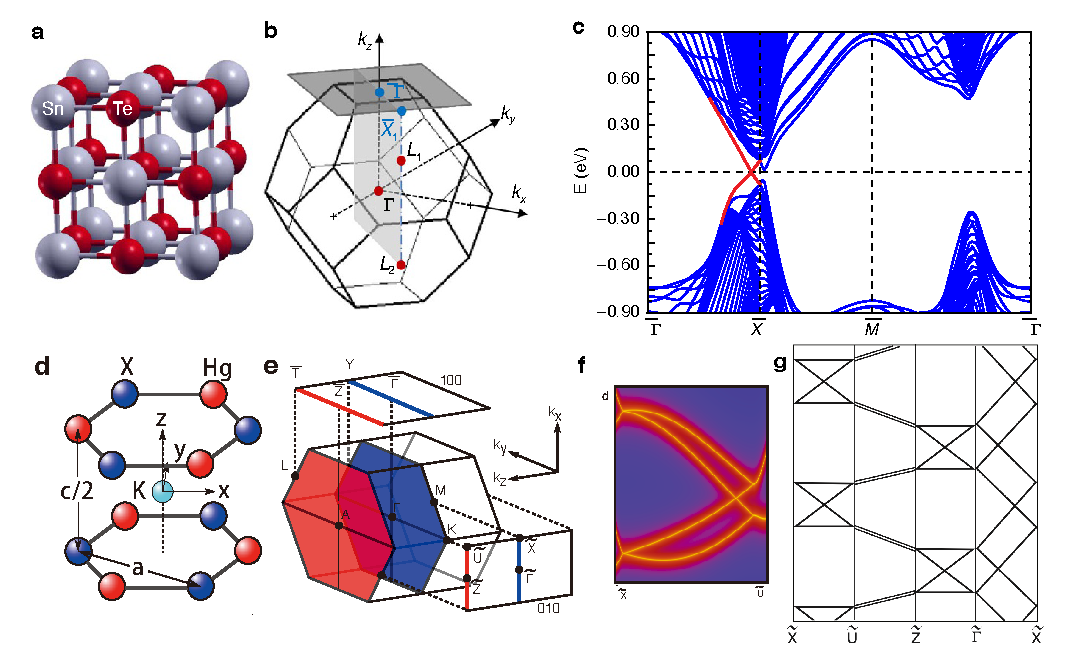
\includegraphics[width=14cm]{chapter1-5.pdf}
    \bicaption{(a)SnTe晶格结构。(b)SnTe的体布里渊区和(001)表面布里渊区。(c)SnTe的(001)表面态。(d)KHg$X$($X$=As, Sb, Bi)的晶体结构。(e)KHg$X$的体布里渊区和(100),(010)表面布里渊区。(f)KHgSb的(010)表面沙漏型色散。(g)不平庸的wilson-loop谱。(图片来自\citep{hsieh2012topological, wang2016hourglass})}
    {(a) SnTe lattice (b) Brillouin zone and [001] surface of SnTe.
    (c) The [001] surface states of SnTe.
    (d) Lattice structure of KHg$X$($X$=As, Sb, Bi).
    (e) bulk Brillouin zone (BZ) of KHg$X$ and 100-surface BZ, 010-surface BZ.
    (f)The dispersion of the hourglass fermion in (010) surface of KHgSb.
    (g)Non-trivial wilson-loop pattern. (From ~\citep{hsieh2012topological, wang2016hourglass})}
    \label{fig:1-5}
\end{figure}
拓扑晶体绝缘体的概念首先由傅亮在2011年提出~\citep{fu2011topological},
他通过紧束缚模型研究了由$C_4$(和$C_6$)旋转对称性加时间反演对称性保护的TCI,并定义了一个新的$\mathbb{Z}_2$不变量。最终发现在保持$C_4$(和$C_6$)不变的(001)表面上,不平庸的$\mathbb{Z}_2$不变量可以保护无能隙的表面态。2012年,傅亮等人又第一次预言了IV–VI族半导体SnTe中可能存在镜面对称性保护的TCI,如图~\ref{fig:1-5} (a-c) , 并且提出PbTe和PbSe经过应力或掺杂后也可以成为TCI~\citep{hsieh2012topological}。同年,角分辨光电子能谱(ARPES)实验很快证实了SnTe和Pb$_{1-x}$Sn$_x$Se中存在由镜面对称性保护的表面狄拉克锥,确实是新型的TCI态~\citep{tanaka2012experimental,Dziawa2012}。这样的体系可以定义的拓扑不变量是镜面陈数。
%,我们会在 (\ref{sec:invariants}) 拓扑不变量这一小节中做详细介绍。

第二个理论预言并在实验上得到验证的是滑移面保护的TCI~\citep{liucx2014,Fang2015new, Shiozaki} -- KHgSb~\citep{wang2016hourglass,ma2017experimental}。这种非简单(non-symmorphic)空间群保护的二维拓扑表面态是一种新奇的沙漏型(hourglass)表面态,如图~\ref{fig:1-5}(d-f),由一个新的$\mathbb{Z}_2$ hourglass拓扑不变量来刻画。由于表面态能谱与Wilson-loop谱是同构的~\citep{fidkowski2011model},也可以计算Wilson-loop谱来判断是否存在不平庸的表面态。如图~\ref{fig:1-5}(g),是表示拓扑不平庸的表面态连接方式,也可以理解为Wilson-loop谱连接方式的示意图。滑移面保护的hourglass表面谱相关性质将在第~\ref{chap:lasbte}章中以LaSbTe为例做更详细的讨论,这里不再赘述。

随后,方辰老师团队又进一步发现了$C_n\mathcal{T}$反常的TCI,在垂直于旋转轴的上下表面分别存在$n$个表面Dirac锥~\citep{songzd2017,Fangc2t},侧表面存在由$C_n$对称性联系起来的棱态,所谓($d-2$)维边界态。其$\mathbb{Z}_2$的拓扑分类可以通过$k_z=0$和$k_z=\pi$面之间瓦尼尔(Wannier)中心的$\mathbb{Z}_2$流来刻画。当然这在实际材料的计算中是很难利用的方法。但是对于同时具有中心反演对称性的体系,可以定义“Fu-Kane-like formula”,直接通过中心反演对称操作的本征值来计算。感兴趣的可以参考原文~\citep{songzd2017,Fangc2t}。后来研究者们也将($d-1$)表面完全开能隙,但是具有($d-2$)维边界态的拓扑晶体绝缘体称为高阶拓扑绝缘体(high-order TI,简称HOTI)~\citep{bernevig17,Schindler,Schindler2018}。2018年,Titus Neupert及其合作者首先预言SnTe经过(110)非轴应力之后可以成为HOTI,即体态和表面态完全开能隙,但是存在由时间反演和镜面对称性保护的螺旋棱态(hinge state)~\citep{Schindler}。同年,他们又理论预言在本征的铋单质(Bismuth,即Bi)中可以出现由空间反演和$C_3$旋转保护的棱态,并通过扫描隧道谱和约瑟夫森干涉实验得到了确凿的实验证据。目前为止,Bi是第一个理论预言并且得到实验验证的高阶拓扑绝缘体~\citep{Schindler2018}。

\begin{figure}[!t]
    \centering
    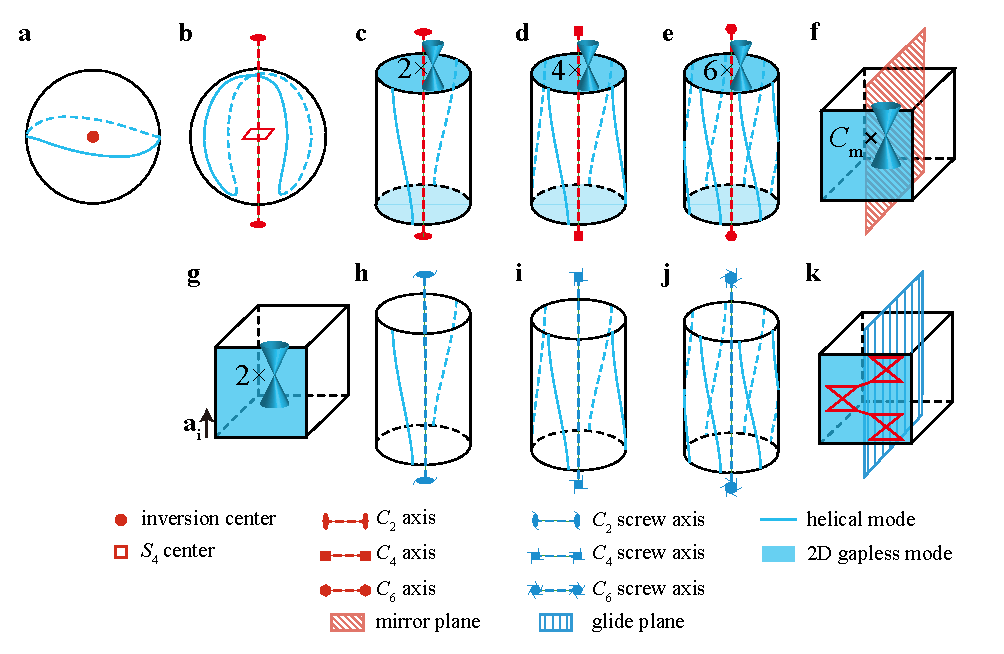
\includegraphics[width=14cm]{chapter1-6.pdf}
    \bicaption{非磁性空间群不同对称性保护的拓扑晶体绝缘体的表面态。由(a)中心反演对称性保护的,(b)S$_4$保护的,(c-e) $C_{n=2,4,6}$旋转对称性保护的,(f)镜面对称性保护的拓扑晶体绝缘体的表面态。(g)弱拓扑绝缘体的表面态。(h-j)$C_{n=2,4,6}$螺旋对称性保护的拓扑晶体绝缘体的表面态。(k)沙漏型的拓扑晶体绝缘体表面态。(图片来自\citep{Song2019})}
    { Surface states of topological crystalline insulators in nonmagnetic space group. The surface state of (a) inversion-protected TCI, (b) S$_4$-protected TCI, (c-e) $C_{n=2,4,6}$-rotation-protected TCI, (f)mirror TCI. (g) The surface state of weak TI. (h-j) The surface states of $C_{n=2,4,6}$-screw-protected TCI. (k) The surface state of hourglass TCI.(From~\citep{Song2019})}
    \label{fig:1-6}
\end{figure}

回顾到此,我们发现镜面对称性,滑移对称性,旋转对称性都可以保护拓扑晶体绝缘体。拓扑晶体绝缘体的完全分类呼之欲出。随着一系列数学物理方法的发展,包括``K-theory",对称性指标理论/拓扑量子化学理论,层构造及实空间构造方法等等,选择一整套可行的方法得到拓扑晶体绝缘体的全部分类似乎是势在必行。2017年底,方辰老师团队首先通过层构造的方法,得到了230个空间群(即第二类磁群)所有的对称性指标和拓扑不变量的映射关系~\citep{song2017}。有了这个映射关系,我们就可以通过简单计算一些对称性指标而获得相对应的可能的拓扑不变量,大大降低了计算的难度。同时这一工作也给出230个空间群中除了
%SG.48, SG.86, SG.134, SG.201 和 SG.224 这五个群是当时用LC方法不能给出所有的indicator。但还有七个群没有indicator,用lc方法不能给出所有的拓扑态。只有用real-space recipe方法之后,才发现这七个态不完整。
Pnn2 (\#34), Pnnn (\#48), P4$_2$ (\#77), P4$_2$/n (\#86), P4$_2$22 (\#93), P4$_2$2$_1$2 (\#94), P4$_2$cm (\#102), P$\bar 4$n2 (\#118), P4$_2$/nnm (\#134), Pn$\bar 3$ (\#201), P4$_2$32 (\#208), 和 Pn$\bar 3$m (\#224)
这12个群之外所有空间群保护的拓扑态~\citep{song2017,Song2019},这使得判断材料具体的拓扑分类成为一件简单的事情。由于非平庸拓扑不变量已经获得,根据体-边对应关系,一定存在不平庸的拓扑表面态。如图~\ref{fig:1-6},显示了不同的拓扑不变量保护的不同表面态构型,包括一些新的拓扑不变量,如螺旋轴不变量保护的螺旋棱态,空间反演对称性和$S_4$不变量保护的棱态。对于层构造方法失效的情况,他们进一步采用局域群保护的拓扑态来替代一个完整二维层构造(2D TI或2D TCI)来装饰每一层(称之为“实空间方法”),最后得到了第二类磁群对称性保护的拓扑晶体绝缘体的全部分类 ~\citep{Song2019}。基于此思想,他们证明了所有由晶体点群对称性保护的拓扑态都可以由更低维度的拓扑态得到,从而给出了拓扑保护的晶体态(包括玻色子和费米子)的完整分类~\citep{Songreal}。
\begin{figure}[!htbp]
    \centering
    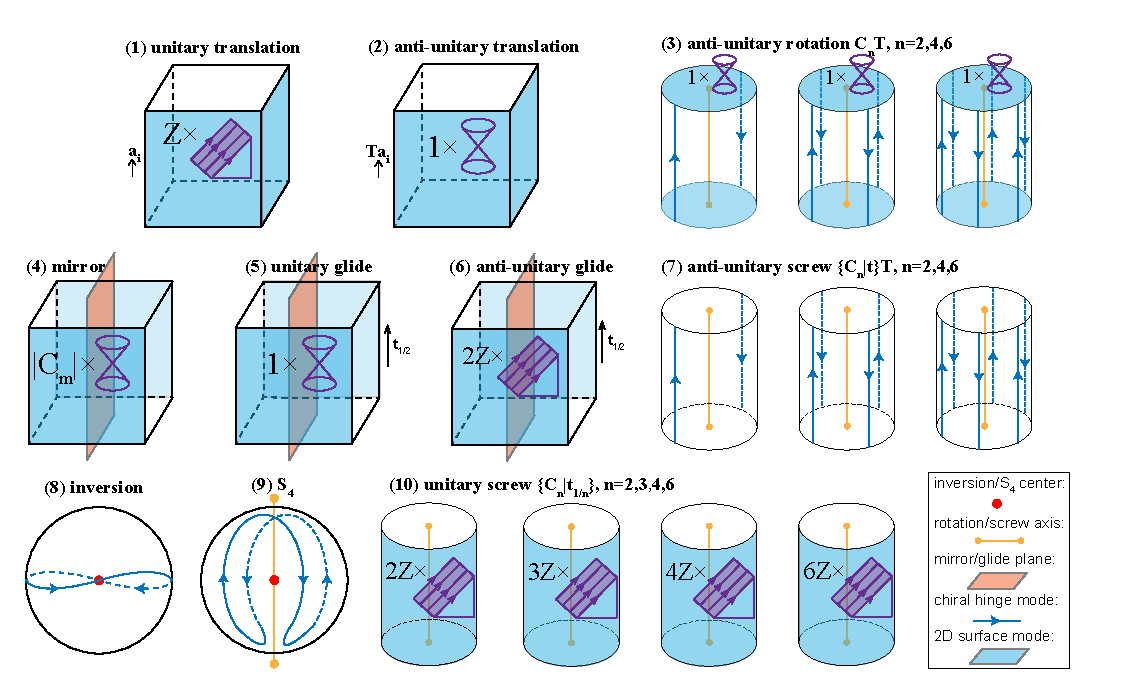
\includegraphics[width=14cm]{chapter1-7.pdf}
    \bicaption{磁空间群的对称操作对应的非平庸拓扑不变量所保护的表面态。二维表面态可以是在(1),(6),(10)中斜坡类型的手性表面态,或者在(2),(3),(4),(5)的狄拉克锥。(图片来自\citep{Peng2021})}
    { Surface states in MSGs, with the corresponding symmetries marked above the plots. The 2D surface modes can be either sloped-like chiral surface modes in (1), (6), (10) or Dirac cones in (2), (3), (4), (5).(From~\citep{Peng2021})}
    \label{fig:1-7}
\end{figure}

2021年年初,方辰老师团队又将“实空间方法”应用到其他三类磁群,给出了每个磁群考虑自旋轨道耦合时的拓扑分类,以及对应的对称性指标和拓扑不变量的映射关系~\citep{Peng2021}。自此完整的分类了所有开能隙的拓扑态。图~\ref{fig:1-7}展示了磁群中不同对称性保护的表面态。除此之外,由于磁群破坏了时间反演对称性,所以会给出一些非磁群不具有的更有意思的结论,比如一些无能隙的拓扑态也可以由不平庸的拓扑不变量来刻画;反幺正的$C_n$旋转对称性给出的表面态是上下只有一个表面狄拉克锥,侧表面的表面态是有$n$个$C_n$对称性联系的手性边界态(chiral hinge mode),而不像非磁性空间群上下表面有$n$个表面狄拉克锥,侧表面有$n$个$C_n$对称性联系的螺旋边界态(helical hinge mode),等等。
相信随着磁性拓扑理论的不断发展~\citep{Elcoro2020,Peng2021},科学家们可以找到更多有意思的材料,如果能够找到一个室温下实现量子反常霍尔效应的材料,必将引领一个新的时代。

\section{拓扑半金属}\label{sec:system}
前面讨论了有能隙的拓扑态,并介绍了这些拓扑态如何进行拓扑分类。那么能否将拓扑分类推广到无能隙的系统呢?我们知道,有能隙的拓扑系统,可以通过占据态的波函数来定义拓扑不变量,因为在布里渊区任意一个$\bold{k}$点,对于绝缘体占据态波函数都有好的定义。但是对于金属而言,不同$\bold{k}$点占据数不同,原来的定义方法就失效了。但是金属不同$\bold{k}$点占据数不同恰好使得其存在费米面,那么我们就可以很自然的利用费米面及其上的波函数来进行拓扑分类。虽然目前为止我们还没有完整分类金属的方法,但是对于半金属,我们可以对其进行分类。因为对于半金属而言,费米面只有一些孤立点或线,而不是一个面,所以可以看作是一种特殊的“绝缘体”。
本论文中,我们主要针对三维空间中三类基本的拓扑半金属:外尔半金属(Weyl Semimetal,即WSM), 狄拉克半金属 (Dirac Semimetal,即DSM), 节点线半金属(Nodal line Semimetal,即NLSM)展开讨论。

\subsection{外尔半金属}\label{sec:weyl}
在三维空间中,两条非简并的能带交叉点附近的低能有效模型一般遵循外尔方程,因而被称为外尔点 (WP)~\citep{1929weyl}。其低能有效哈密顿量形如:
\begin{equation}
    \label{eq:1-6}
    H(\mathbf{k})= \pm \mathbf{k} \cdot \sigma
\end{equation}
然后,我们可以定义包裹外尔点的费米面上的陈数:
\begin{equation}
    \label{eq:1-7}
    C_{\mathrm{FS}}=\frac{1}{2 \pi} \int_{\mathrm{FS}} \boldsymbol{\Omega}(\mathbf{k}) \cdot \mathrm{d} \mathcal{S}
\end{equation}
其中,$\Omega_{\pm}(\mathbf{k})=\mp \frac{\mathbf{k}}{2|k|^{3}}$是贝利曲率,可以看作动量空间的磁场,那么外尔点就可以理解为动量空间的磁单极子。陈数$C_{\mathrm{FS}}=\pm 1$就对应包裹的外尔点的手性为+1或-1。这是描述外尔点的拓扑不变量。
根据“no-go”定理~\citep{NIELSEN198120,NIELSEN1981173},相反手性的外尔点总是成对出现的,在动量空间总陈数为0。
三维空间中三个泡利矩阵是完备基,所以由方程~\ref{eq:1-6}可以看到,这样一个哈密顿量无法加入任何质量项。微扰只能移动外尔点,但不能把它开能隙,除非将两个相反手性的外尔点移动到一起。所以除了要求动量是好的量子数,即只须要求满足平移对称性外不需要其他任何对称性保护,外尔半金属则可以稳定存在。另外,如果体系有其他对称性时,比如$C_4$,$C_6$旋转或者螺旋对称性,外尔点还可以携带更高手性的电荷,此时垂直于旋转轴的色散也不再是简单的线性色散,而是二次型或者三次型色散~\citep{Fang2012,Tsirkin2017}。
那么在三维体系中如何实现这样两重简并的外尔点呢?我们知道如果时间反演$\mathcal{T}$和空间反演$\mathcal{P}$对称性同时存在时,每条能带两重简并,所以这时候的能带交叉点总是相当于两个外尔点相遇在一起。所以要想得到外尔点,我们必须破坏空间反演对称性$\mathcal{P}$,或者时间反演对称性$\mathcal{T}$中的一个。第一种情况对应于非磁性的外尔半金属,第二种情况则对应于磁性外尔半金属。下面我们将对这两种情况加以讨论。

\begin{figure}[!htbp]
    \centering
    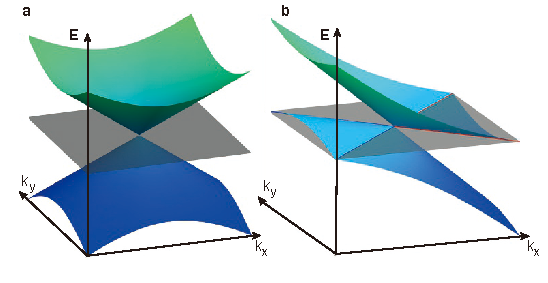
\includegraphics[width=14cm]{chapter1-8.pdf}
    \bicaption{外尔半金属可能的类型。(a)有点状费米面的第一类外尔半金属。(b)出现在电子口袋和空穴口袋接触点的第二类外尔半金属。灰色的面代表费米能级,蓝色(红色)的线代表空穴(电子)口袋的边界。(图片来自\citep{soluyanov2015type})}
    { Possible types of Weyl semimetals. (a) Type-I WP with a pointlike Fermi surface. (b) A type-II WP appears as the contact point between electron and hole pockets. The grey plane corresponds to the position of
    the Fermi level, and the blue (red) lines mark the boundaries of the hole
    (electron) pockets.(From~\citep{soluyanov2015type})}
    \label{fig:1-8}
\end{figure}

对于非磁性外尔半金属,体系内外尔点的数目总是4的倍数。因为如果在动量$\mathbf{k}$处存在一个外尔点,那么由于时间反演对称性使得在动量$-\mathbf{k}$处也存在一个相同手性的外尔点。根据体系中总的外尔点陈数为0,可以知道,一定有另外两个手性相反的外尔点同时存在。非磁性外尔半金属可以看作是拓扑绝缘体到普通绝缘体的相变点~\citep{Murakami_2007,Murakami2}。因为从拓扑绝缘体到普通绝缘体的相变的过程中一定要发生能带反转,而且能带反转前后,占据态的中心反演本征值发生改变,才能带来拓扑的不同~\citep{Fu2007IS},所以能带反转过程中出现的交叉点一定具有不同的中心反演本征值而保证能隙不被打开。这个交叉点就是外尔点。
根据形成外尔点的两条能带的费米速度不同,我们可以将外尔半点分为两种类型,Type I 和Type II~\citep{soluyanov2015type} 。如方程~\ref{eq:1-6}, 一般情况下是点状费米面,如图~\ref{fig:1-8} (a) 所示,我们称这种外尔点是Type I 外尔点。著名的TaAs家族即属于这类。但是在实际材料中,也存在外尔点出现电子口袋和空穴口袋的边界上,如图~\ref{fig:1-8} (b) 所示,我们称这种外尔点是Type II 外尔点,如WTe$_2$, MoTe$_2$。虽然费米速度不同,但是Type II外尔半金属也同样如第一类半金属一样,存在特有的费米弧(Fermi arc)表面态,费米弧连接在表面布里渊区的两个外尔点的投影。但是与此同时,又因为费米面附近不同的态密度,使得Type II外尔半金属又具有不同于Type I外尔半金属的一些新奇的物理性质,如由于动量空间的Klein隧道导致的新奇的量子振荡现象,修正的反常霍尔电导等~\citep{soluyanov2015type,Brien2016}。

对于磁性外尔半金属,允许最少出现两个外尔点。因为如果在动量$\mathbf{k}$处存在一个外尔点,那么由于空间反演对称性使得在动量$-\mathbf{k}$处也存在一个相反手性的外尔点,此时两个外尔点即可满足“no-go”定理。对于一个铁磁性外尔半金属,考虑一个玩具模型~\citep{Armitage2018}:
\begin{equation}
    \label{eq:1-8}
    \begin{aligned}
    H(\mathbf{k})=& t_{z}\left(2-\cos k_{x} a-\cos k_{y} a+\gamma-\cos k_{z} a\right) \sigma_{z}\\
    &+t_{x}\left(\sin k_{x} a\right) \sigma_{x}+t_{y}\left(\sin k_{y} a\right) \sigma_{y}
    \end{aligned}
\end{equation}
这里假设基矢轨道具有相反的宇称,所以$\mathcal{P}=\sigma_{z}$。当$-1<\gamma<1$时,此时宇称相反的能带发生反转,存在一对外尔点位于$(0,0,\pm k_0)$,其中$\cos(k_0)=\gamma$。此时除了$k_z=\pm k_0$的面之外,布里渊区其他$k_z$平面内没有能带简并点,可以定义陈数$\Omega(k_z)$。计算发现$\Omega(|k_z|> k_0)=0$, $\Omega(|k_z|< k_0)=1$。可见外尔点出现在一系列二维陈绝缘体和普通绝缘体之间。所以外尔半金属可以看作是陈绝缘体的三维“强”拓扑态~\citep{weng2015quantum}。总的霍尔电导计算可得$\sigma_{xy}=\frac{e^2}{\pi h} k_0$。所以在铁磁外尔半金属中也可以期望反常霍尔效应的出现。
当化学势恰好在两个外尔点上时,此时费米面是两个点。随着化学势增大,费米面逐渐增大,体系总的霍尔电导逐渐减小,这因为上面能带对贝利曲率的贡献与下面的能带贡献相互抵消所致。当化学势增大到两条能带完全被占据,总的霍尔电导就被完全抵消为零。所以,理想情况下,我们总是希望化学势恰好穿过费米面~\citep{weng2015quantum,Armitage2018}。

外尔半金属因为包裹外尔点的陈数不为零,根据体-边对应关系,可得外尔半金属也一定存在不平庸的表面态。
表征外尔半金属的一个很重要特点就是在表面态上有连接两个外尔点的费米弧。根据上面讨论可知,外尔半金属可以看作由许多二维陈绝缘体和普通绝缘体的堆叠,而这个费米弧的出现也可以看作是这些陈绝缘体的手性边界态。这一特点可以通过ARPES实验来测量。除此之外,外尔半金属还有许多新奇的可观测效应,如手性反常,负磁阻现象,手性磁效应,弱反局域化等等。

材料方面,2011年,南京大学万贤刚老师团队首先在烧绿石铱酸盐提出第一个磁性外尔半金属~\citep{Wan2011}。同年物理所方忠老师团队,预言在铁磁结构HgCr$_2$Se$_4$中存在拓扑电荷为2的双重外尔点~\citep{xu2011chern}。
但是由于ARPES在磁性材料方面测量困难,2014年底,物理所翁红明老师团队首次提出TaAs家族是空间反演对称性破缺的非磁性外尔半金属~\citep{weng2015weyl},很快便得到实验证实~\citep{lv2015experimental,lv2015observation,lv2015observation2}。几乎同时期,普林斯顿研究团队也预言并实验确认了这个材料是外尔半金属~\citep{huang2015weyl,xu2015discovery,xuSY2015}。由于TaAs在样品制备和实验测量方面的优势,目前为止仍然是研究外尔半金属的明星材料。 最近,科学家们又预言了层状Kagome结构铁磁Co$_3$Sn$_2$S$_2$和层状铁磁MnBi$_2$Te$_4$是铁磁外尔半金属~\citep{cosns2018,xucosns,zhanghj2019,Li2019}。并且Co$_3$Sn$_2$S$_2$被观察到巨大的内秉反常霍尔效应~\citep{cosns2018,2017Giant},成为第一个在实验上确认的磁性外尔半金属,这必将为外尔半金属和反常霍尔效应的发展带来更多新的突破。


\subsection{狄拉克半金属}\label{sec:dirac}
狄拉克半金属是一类其低能激发可以用赝相对论狄拉克费米子描述的相。对于一个同时具有时间反演$\mathcal{T}$和空间反演对称性$\mathcal{P}$的体系,动量空间的每一个点必然具有克拉默简并(Kramers' pair),那么两对外尔点就会重合在一起,形成一个四重简并点。那么描述这样一个具有线性色散的简并点的系统至少需要$4\times4$的哈密顿量:
\begin{equation}
    \label{eq:1-9}
    H(\mathbf{k})=\left[\begin{array}{cc}
    \mathbf{k} \cdot \boldsymbol{\sigma} & 0 \\
    0 & -\mathbf{k} \cdot \boldsymbol{\sigma}
    \end{array}\right]
\end{equation}
满足这个方程的无能隙的交叉点,称之为狄拉克点。因为包裹狄拉克点的费米面上的陈数为0,这个简并点是不受拓扑保护的。
显然,方程~\ref{eq:1-7}很容易通过加入一个质量项打开能隙,所以三维狄拉克点并不稳定。事实上,DSM可以看作是普通拓扑绝缘体到拓扑绝缘体相变过程的临界点。根据Murakami等人的理论~\citep{Murakami_2007,Murakami2},总是可以调节外部参数$m$使得当$m=m_c$时,发生相变。但是从这里也可以看出,一旦$m\neq m_c$,狄拉克点将不复存在。
所以要保证狄拉克点稳定存在,则必须考虑额外的晶体对称性,如$n$度旋转对称性$C_{n=2,3,4,6}$,从而使得狄拉克半金属的相变区间不再是一个点。
%%

\begin{table}[!htbp]\footnotesize
    \centering
    \caption{第一类三维狄拉克半金属。(表格来自~\citep{Yang2014})}
    {Classification of Type I 3D Dirac semimetal. (From~\citep{Yang2014})}
    \label{table:1-1}
    %\resizebox{\textwidth}{15mm}{
    \setlength{\tabcolsep}{0.5mm}{
    \begin{tabular}{c c c c c c c c c c c c c c c}
    \hline
%    \hline
    $C_{n}$ & & $|P|$& &$(u_{A,\uparrow},u_{B,\uparrow})$ & & f($k_{\pm}$, $k_{z}$) & & g($k_{\pm}$, $k_{z}$)  & & 2D topological invariant & & $H_{\text{Dirac}}(\textbf{q})$ && Materials\\
    \hline
%    \hline
    $C_{2}$ & & $\tau_{z}$ & & $-$ & & $-$ & & $-$ & & $-$  & & Not allowed & &\\
    $C_{2}$ & & $\tau_{0}$ & & $-$ & & $-$ & & $-$ & & $-$  & & Not allowed & &\\
%    \hline
%    \hline
    $C_{3}$ & & $\tau_{z}$ & &$(e^{i\pi},e^{i\frac{\pi}{3}})$ & & $\beta k_{+}$ & & $\gamma k_{-}$  & & $\nu_{2D}=1$ & & Linear Dirac & & Na$_{3}$Bi\\
    &&&&&&&&&&&&&&~\citep{wang2012dirac} \\
    $C_{3}$ & & $\tau_{0}$ & &$(e^{i\pi},e^{i\frac{\pi}{3}})$ & & $\beta k_{z}k_{+}+\gamma k_{-}^{2}$ & & $\eta k_{z}k_{-}+\xi k_{+}^{2}$  & &$\nu_{2D}=0$ & & Linear Dirac& &\\
%    \hline
%    \hline
    $C_{4}$ & & $\tau_{z}$ & &$(e^{i\frac{3\pi}{4}},e^{i\frac{\pi}{4}})$ & & $\eta k_{+}$ & & $\beta k_{z}k_{+}^{2}+\gamma k_{z}k_{-}^{2}$  & & $n_{M}=\pm1$ & & Linear Dirac
    & & Cd$_{3}$As$_{2}$\\
    &&&&&&&&&&&&&&~\citep{wang2013three} \\
    $C_{4}$ & & $\tau_{0}$ & &$(e^{i\frac{3\pi}{4}},e^{i\frac{\pi}{4}})$ & & $\eta k_{z}k_{+}$ & & $\beta k_{+}^{2}+\gamma k_{-}^{2}$  & &
    $n_{M}=2\text{sgn}(|\beta|-|\gamma|)$ & & Linear Dirac & &\\
%    \hline
%    \hline
    $C_{6}$ & & $\tau_{z}$ & &$(e^{i\frac{\pi}{2}},e^{i\frac{\pi}{6}})$ & & $\beta k_{+}$ & & $\gamma k_{z}k_{+}^{2}$ & & $n_{M}=\pm1$ & & Linear Dirac & &\\
    $C_{6}$ & & $\tau_{0}$ & &$(e^{i\frac{\pi}{2}},e^{i\frac{\pi}{6}})$ & & $\beta k_{z}k_{+}$ & & $\gamma k_{+}^{2}$ & & $n_{M}=\pm2$ & & Linear Dirac & &\\
%    \hline
    $C_{6}$ & & $\tau_{z}$ & &$(e^{i\frac{5\pi}{6}},e^{i\frac{\pi}{2}})$ & & $\beta k_{+}$ & & $\gamma k_{z}k_{-}^{2}$ & & $n_{M}=\pm1$ & & Linear Dirac & &\\
    $C_{6}$ & & $\tau_{0}$ & &$(e^{i\frac{5\pi}{6}},e^{i\frac{\pi}{2}})$ & & $\beta k_{z}k_{+}$ & & $\gamma k_{-}^{2}$ & & $n_{M}=\pm2$ & & Linear Dirac & &\\
%    \hline
    $C_{6}$ & & $\tau_{z}$ & &$(e^{i\frac{5\pi}{6}},e^{i\frac{\pi}{6}})$ & & $\eta k_{z}k_{+}^{2}$ & &$\beta k_{+}^{3}+\gamma k_{-}^{3}$ & &
    $n_{M}=3\text{sgn}(|\beta|-|\gamma|$) & & Quadratic Dirac & &\\
    $C_{6}$ & & $\tau_{0}$ & &$(e^{i\frac{5\pi}{6}},e^{i\frac{\pi}{6}})$ & & $\eta k_{+}^{2}$ & &$\beta k_{z}k_{+}^{3}+\gamma k_{z}k_{-}^{3}$ & & $n_{M}=\pm2$
    & & Quadratic Dirac & &\\
%    \hline 
    \hline
    \end{tabular}
    }
\end{table}
%%
%%%%
\begin{table}[!htbp]\small
    \centering
    \caption{第二类三维狄拉克半金属。(表格来自~\citep{Yang2014})}
    {Classification of Type I 3D Dirac semimetal. (From~\citep{Yang2014})}
    \label{table:1-2}
    %\resizebox{\textwidth}{15mm}{
    \setlength{\tabcolsep}{0.5mm}{
    \begin{tabular}{c c c c c c c c c c c c c}
%    \hline
    \hline
    $C_{n}$ & & $|P|$& &$u_{A,\uparrow}$ & & f($k_{\pm}$, $k_{z}$) & & $g_{z}$($k_{\pm}$, $k_{z}$)   & & $H_{\text{Dirac}}(\textbf{q})$ && Material\\
    \hline
%    \hline
    $C_{2}$ & & $\tau_{x}$ & & $e^{i\frac{\pi}{2}}$ & & $k_{z}F_{1}^{(1)}(k_{x,y})-iF_{2}^{(1)}(k_{x,y})$
    & & $\alpha k_{x}+\beta k_{y}$   & & Linear Dirac && Distorted Spinels\\
    &&&&&&&&&&&&~\cite{spinels}\\
%    ccccccccccccc
%    \hline
%    \hline
    $C_{3}$ & & $\tau_{x}$ & &$-$ & & $-$ & & $-$   & & Not allowed &&\\
%    \hline
%    \hline
    $C_{4}$ & & $\tau_{x}$ & &$e^{\pm i\frac{\pi}{4}}$ & & $F_{1}^{(2)}(k_{x,y})-ik_{z}F_{2}^{(2)}(k_{x,y})$
    & & $\alpha k_{\pm}$   & & Linear Dirac&& BiO$_{2}$\\
    &&&&&&&&&&&&~\cite{Young12}\\
%    \hline
%    \hline
    $C_{6}$ & & $\tau_{x}$ & &$e^{\pm i\frac{\pi}{6}}$ & & $k_{z}F_{1}^{(3)}(k_{x,y})
    +iF_{2}^{(3)}(k_{x,y})$ & & $\alpha k_{\pm}$  & & Linear Dirac &&\\
%    \hline
    $C_{6}$ & & $\tau_{x}$ & &$e^{i\frac{3\pi}{6}}$ & & $k_{z}F_{1}^{(3)}(k_{x,y})
    +iF_{2}^{(3)}(k_{x,y})$ & &$F_{3}^{(3)}(k_{x,y})
    +iF_{4}^{(3)}(k_{x,y})$
    & & Cubic Dirac &&\\
    \hline 
    %\hline
    \end{tabular}}
\end{table}
%%%

根据狄拉克点的位置,可以将DSM分为两类~\citep{Yang2014}:
一类是由于能带反转造成的偶然简并点,使得在旋转轴上存在一对狄拉克点的Type I DSM,如Na$_3$Bi~\citep{wang2012dirac},Cd$_3$As$_2$~\citep{wang2013three}。
%, 此时对称操作满足$\{C_n$,$\mathcal{P}\}$=0。
另一类是由于“对称性强制(symmetry-enforced)”而产生的,只在单个时间反演不变点上存在狄拉克点的Type II DSM,如BiO$_2$~\citep{Young12},扭曲尖晶石~\citep{spinels}。
%,此时对称操作满足[$C_n$,$\mathcal{P}$]=0;
对于第一类由于偶然简并造成的DSM相,可以定义拓扑不变量来进行刻画。因为狄拉克点只在旋转轴上存在,我们可以在$k_z=0$的完全开能隙的面内计算$\mathbb{Z}_2$(或者如果$k_z=0$是镜面, 可计算镜面陈数$n_M$)。狄拉克半金属的两种不同的分类分别列在表格~\ref{table:1-1},~\ref{table:1-2}中。
对于具有非平庸拓扑不变量的狄拉克半金属,根据体-边对应关系,则存在不平庸的拓扑表面态~\citep{Yang2014}。




%\clearpage
\subsection{节点线半金属}\label{sec:nlsm}
节线半金属是区别于外尔半金属和狄拉克半金属的另外一类半金属,其能带简并点在动量空间中是一维的线而非单个孤立的点~\citep{burkov2011}。节线半金属可以在二维系统,也可以在三维系统中存在。我们只讨论三维系统的节线半金属。

根据不同的对称性,节线半金属可以做不同的分类。
在不考虑自旋轨道耦合的情况下,有分别由中心反演和时间反演的组合对称性$\mathcal{PT}$,镜面对称性$M$,非简单空间群对称性$\tilde{g}$这三种对称性保护的三类节线半金属~\citep{fang2015nl,Fang2016cpb}。这三类节线半金属都是外尔节线半金属,即简并点两重简并。在同时存在某些对称性的情况下,也可以出现狄拉克节线半金属,即简并点是四重简并。这种非自旋轨道耦合的狄拉克节线半金属只能出现在空间群57,60,61,62,205这五个空间群里,我们不再做详细讨论,感兴趣的可以参考文献~\cite{Li2021,Yu2021}。$\mathcal{PT}$保护的节线半金属的拓扑分类是$\mathbb{Z}_2$的,因为其波函数的一阶和二阶同伦群都是$\mathbb{Z}_2$。最简单的,我们可以考虑一个两带模型:
\begin{equation}
    \label{eq:1-10}
    H_{0}(\mathbf{k})=g_{x}(\mathbf{k}) \sigma_{x}+g_{y}(\mathbf{k}) \sigma_{y}+g_{z}(\mathbf{k}) \sigma_{z}
\end{equation}
其中$\mathcal{PT}=\mathcal{K}$, $\mathcal{K}$是复共轭算符, 所以$g_{y}=0$。简并点由$g_{x}=g_{z}=0$决定。两个方程,三个未知数,所以解在三维空间中一定是一维的线。当把系统加倍$H_{d}=H_{0}(\mathbf{k}) \oplus H_{0}(\mathbf{k})=s_{0} \otimes H_{0}(\mathbf{k})$,我们发现可以加入一个保持$\mathcal{PT}$对称性的质量项$m s_{y} \sigma_{y}$来打开能隙,这就说明这个节线半金属是$\mathbb{Z}_2$分类的。此时可以定义一个穿过节线半金属的闭环,如图~\ref{fig:1-9} (a) ,计算环绕闭环一周的贝利相位,这个贝利相位就是这类节线半金属的$\mathbb{Z}_2$不变量~\citep{kim2015nl}。这类节线半金属可以通过调节参数使得其收缩为一点,最终完全消失,如图~\ref{fig:1-9} (c) 。
\begin{figure}[!htbp]
    \centering
    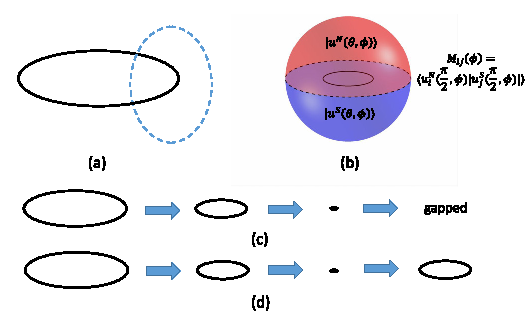
\includegraphics[width=10cm]{chapter1-9.pdf}
    \bicaption{(a)不平庸$\mathbb{Z}_2$不变量:贝利相位$\pi$。(b)对于拓扑不变量定义在球面的节线半金属的2维$\mathbb{Z}_2$不变量。(c)由方程(1.10)描述的零单极电荷的节线半金属的演化。(d)由方程(1.11)描述的有单极电荷的节线半金属随着参数调节的演化。(图片来自\citep{fang2015nl})}
    { (a) A nontrivial $\mathbb{Z}_2$ invariant (Berry’s phase of π) of any loop in 3D BZ implies a nodal line (solid line) passing through the loop. (b) The 2D $\mathbb{Z}_2$ invariant for a nodal line in 3D BZ defined on a sphere enclosing the line. (c) The evolution of a nodal line with zero monopole charge as the parameter changes in the model of Eq. (1.10). (d) The evolution of a nodal line with nonzero monopole charge as the parameter changes in the model of Eq. (1.11). (From~\citep{fang2015nl})}
    \label{fig:1-9}
\end{figure}
方辰老师等人还发现,$\mathcal{PT}$对称性还能保护另外一类$\mathbb{Z}_2$类型的节线半金属,其拓扑不变量由定义在包裹该节线半金属的球面上的$\mathbb{Z}_2$数来决定,如图~\ref{fig:1-9} (b) ~\citep{fang2015nl,Fang2016cpb}。描述这样的一种节线半金属的哈密量可以写作:
\begin{equation}
    \label{eq:1-11}
    H_{0}(\mathbf{k})=k_{x} \sigma_{x}+k_{y} \tau_{y} \sigma_{y}+k_{z} \sigma_{z}+m \tau_{x} \sigma_{x}
\end{equation}
这个哈密顿量描述了一个在$k_z=0$面内半径为$\sqrt{|m|}$的节线环。当调节参数$m$从正数变为负数的过程中, 我们发现节线环会先缩为一点,然后又变回一个节线环,而不会消失,如图~\ref{fig:1-9}(d)。这样的节线半金属只能通过与另一个
$\mathbb{Z}_2$荷相同的节线环相遇才能消除掉。如果把两个方程~\ref{eq:1-11}描述的节线环直和起来$H_{d}=s_{0} \otimes H_{0}(\mathbf{k})$,仍然可以找到一个满足$\mathcal{PT}$对称性的质量项$m^{\prime} s_{0} \tau_{x} \sigma_{y}$,使得节线环不能稳定存在。所以这样的节线环仍然是$\mathbb{Z}_2$分类的。$\mathcal{PT}$保护的节线半金属往往在一般位置上,因而不太容易确定。为此,方辰老师团队发展了一套对称性指标理论,可以确定节线半金属的构型和可能的位置,为理解节线半金属成因和寻找节线半金属起到了重要的作用~\citep{song2018nl}。

不同于$\mathcal{PT}$对称性保护的节线半金属,镜面保护的节线半金属是$\mathbb{Z}$的拓扑分类,同样可以利用上面的“质量项”的方法进行分析,感兴趣的读者可以参考~\citep{chiu2014}。~\cite{chiu2014}文章详细讨论了由镜面对称性保护的节线半金属的拓扑分类问题。当镜面对称性与其他对称性,如时间反演,粒子-空穴对称性,手性对称性等,同时出现时,镜面对称性还会将原本“十重类”(“tenfold-class”)丰富到27类不同的拓扑分类。~\cite{chiu2014}文章同时还给出了由镜面对称性相联系的不处于镜面上的节线半金属的分类。

在考虑自旋轨道耦合的情况下,单独由$\mathcal{PT}$对称性则不再能保护节线半金属。因为我们知道,此时由于克拉默对的存在,每条能带在每个$\mathbf{k}$点都是两重简并的。所以必须考虑更多的对称性,从而形成狄拉克节线半金属。这种情况相对复杂,可以参考文献~\cite{fang2015nl,liang2016,chen2016,shao2020,wu2020}。而对于破坏空间反演$\mathcal{P}$或者时间反演$\mathcal{T}$对称性的节线半金属情况则较为简单,此时单独的镜面对称性或者非简单空间群对称性就可以保护外尔节线半金属,其情况与不考虑自旋轨道耦合时相似,比如在考虑自旋轨道耦合时,Pb(Tl)TaSe$_2$就是典型的镜面对称性保护的非中心对称的外尔节线半金属~\citep{TlTaSe,Bian2016}。表格~\ref{table:1-3}给出了一些典型的节线半金属材料的拓扑分类~\citep{Fang2016cpb}。

和其他拓扑态一样,由体-边对应关系,节线半金属中非平庸的拓扑不变量也会保证表面态的出现。不同于外尔半金属只有零维的无能隙点,节线半金属无能隙的点是一维的线,所以其表面态构型也大不相同。节线半金属的表面态是连接所有无能隙交叉点的平带,由于在三维动量空间中形如鼓膜,也称为“鼓膜态”。如果体系中存在额外对称性时,如手性对称性,节线半金属的表面态是零能的鼓膜态。但是一旦施加一个化学势,鼓膜态就不再是严格的零能态,而是会具有一定的色散。这种新奇的表面态的存在也使得节线半金属具有很多新奇的物理性质,如特别的朗道能级和光电导行为\citep{landau,2016Optical}。
%以$\mathcal{PT}$保护的第一类$\mathbb{Z}_2$不平庸的节点环为例,由于节线半金属中无能隙的点是一维的线(或环),所以-“鼓膜态”(drumhead edge states)。

\begin{table}\small
    \centering
    \caption{一些被理论或者实验认为是节线半金属的材料及其分类。(表格来自\citep{Fang2016cpb})}
    {The proposed materials to host nodal lines classified. The DSM, WSM and TI mean the nodal lines evolve into the corresponding topological state when spin-orbit coupling (SOC) is further included. N/A means unknown. Type-A means that the nodal lines are protected by mirror reflection symmetry; type-B means that the nodal lines are protected by space inversion and time-reversal symmetry; type-C means the existence of dirac-nodal lines. (From~\citep{Fang2016cpb})}
    \label{table:1-3}
%    \resizebox{\textwidth}{15mm}{
    \setlength{\tabcolsep}{0.8mm}{    
    \begin{tabular}{c c c}
    \hline
 %   \hline
    Class   & NO SOC  &  +SOC  \\
         \hline
    Type A & TaAs, ZrTe 				& Weyl semimetal \\
                & CaAg$X$ ($X$=P, As) 	& Topological insulators\\
                &						& HgCr$_2$Se$_4$, TlTaSe$_2$, PbTaSe$_2$\\
%         \hline
    Type B 	& CaP$_3$ & Topological insulators \\
            & MTC, BaSn$_2$, BP, IGN, BCO-C$_{16}$	& Topological insulators\\
            & Be and other alkaline-earth metal, Ca$_3$P$_2$ & N/A\\
            &Cu$_3$(Pd, Zn)N, LaN, CaTe	& Dirac semimetals\\
%         \hline
    Type C &  & SrIrO$_3$, Ba$M$$X_3$ ($M$=V, Nb, Ta, $X$=S, Se) \\
         \hline
%         \hline
    \end{tabular}
    }
\end{table}
    
\section{拓扑材料的判别方法}\label{sec:topodiag}
在本章的前几节我们已经介绍了拓扑理论的背景和一些目前为止已经发现的拓扑态。那如何判断一个体系是否具有拓扑,具有什么样的拓扑呢?最近的拓扑量子化学方法/对称性指标理论和实空间构造的方法的发展就可以很好的解答这两个问题。在本节,我们将简单介绍这几个理论。
%,然后介绍一些常见的拓扑不变量的计算方法。

%脆拓扑,用twisted-boundary conditions~\citep{Song2020}
\subsection{拓扑量子化学和对称性指标理论}
通过元素之间的离子键或共价键描述的绝缘化合物的共同特点是,他们的基态波函数可以绝热地变形为电子局域在原子或原子间的乘积态(局域的瓦尼尔函数)。 这种情况即是拓扑平庸态,称之为原子绝缘体 (atomic insulator, 简称AI) 或者基本能带表示(elementary band representation,简称EBR)。那么,很自然地,如果一个体系占据态的波函数可以等价于一些局域的瓦尼尔函数,那么这个系统就是平庸的。反之,如果存在拓扑阻塞,那么这个系统就是具有拓扑的。这便是拓扑量子化学和对称性指标理论的核心思想~\citep{nc_ashvin,tqc2017}。所谓的AI,就是在实空间的最大Wyckoff位置(maximum Wyckoff position)上放原子轨道,要求所放的原子轨道满足相应Wyckoff位置小群的对称性,由此诱导得到的不等价的表示(的数目)可以构成一个有限的阿贝尔群,我们可以将其记为$\{\textrm{AI}\}$(或EBR)。 针对某个空间群对应的有能隙的系统,我们可以再定义一个群$\{\textrm{BS}\}$,即在满足相容性关系的前提下,由所有占据态能带的最大$\mathbf{k}$点上的表示(数目)构成的群。那么判断一个系统是否拓扑,就简化为比较两个群$\{\textrm{AI}\}$,$\{\textrm{BS}\}$之间的关系,在数学上,如果$\{\textrm{AI}\} \le \{\textrm{BS}\}$成立,就等价于计算二者的商群:
\begin{equation}
    \label{eq:1-12}
    X_{\mathrm{BS}} \equiv \frac{\{\mathrm{BS}\}}{\{\mathrm{AI}\}}
\end{equation}
Watanabe团队~\citep{nc_ashvin}发现,在230个空间群,无论是否考虑自旋轨道耦合和时间反演对称性,$\{\textrm{BS}\}$的维度$d_{\mathrm{BS}}$和$\{\textrm{AI}\}$的维度$d_{\mathrm{AI}}$总是满足$d_{\mathrm{BS}}=d_{\mathrm{AI}}$。所以商群总是个有限群:
\begin{equation}
    \label{eq:1-13}
    X_{\mathrm{BS}}=\mathbb{Z}_{s_{1}} \times \mathbb{Z}_{s_{2}} \times \ldots \times \mathbb{Z}_{s_{d_{\mathrm{BS}}}}
\end{equation}
只要$s_{i}>1$,体系就是拓扑的~\citep{nc_ashvin,Po2020}。
基于此,得到所有空间群的有无自旋轨道耦合和时间反演对称性情况下的拓扑分类,如表格~\ref{tab:Spinful_TRX}和表格~\ref{tab:Spinless_TRX}~\citep{nc_ashvin}。
%%%
%%%%%%%%

\begin{table}[h]\small
    \centering
    \caption{考虑时间反演对称性和自旋轨道耦合的系统的对称性指标。(表格来自\citep{nc_ashvin})}
    {\bf Symmetry-based indicators of band topology for systems with time-reversal symmetry and significant spin-orbit coupling. (From~\citep{nc_ashvin})
    \label{tab:Spinful_TRX}}
    \begin{tabular}{c c} \hline 
    $X_{\rm BS}$ & Space groups \\
    \hline
    $\mathbb Z_{2}$  &  81, 82, 111, 112, 113, 114, 115, 116, 117,118\\
     &119, 120, 121, 122, 215, 216, 217, 218, 219, 220\\
%    \hline
    $\mathbb Z_{3}$  &  188, 190\\
%    \hline
    $\mathbb Z_{4}$  &  52, 56, 58, 60, 61, 62, 70, 88, 126, 130, 133, 135, 136, 137, 138,\\
                     &  141, 142, 163, 165, 167, 202, 203, 205, 222, 223, 227, 228, 230\\
%    \hline
    $\mathbb Z_{8}$  &  128, 225, 226\\
%    \hline
    $\mathbb Z_{12}$  &  176, 192, 193, 194\\
%    \hline
    $\mathbb Z_{2} \times \mathbb Z_{4}$  &  14, 15, 48, 50, 53, 54, 55, 57, 59, 63, 64, 66, 68, 71, 72\\
    & 73, 74, 84, 85, 86, 125, 129,131, 132, 134, 147, 148\\
     & 162, 164, 166, 200, 201, 204, 206, 224\\
%    \hline
    $\mathbb Z_{2} \times \mathbb Z_{8}$  &  87, 124, 139, 140, 229\\
%    \hline
    $\mathbb Z_{3} \times \mathbb Z_{3}$  &  174, 187, 189\\
%    \hline
    $\mathbb Z_{4} \times \mathbb Z_{8}$  &  127, 221\\
%    \hline
    $\mathbb Z_{6} \times \mathbb Z_{12}$  &  175, 191\\
%    \hline
    $\mathbb Z_{2} \times \mathbb Z_{2} \times \mathbb Z_{4}$  &  11, 12, 13, 49, 51, 65, 67, 69\\
%    \hline
    $\mathbb Z_{2} \times \mathbb Z_{4} \times \mathbb Z_{8}$  &  83, 123\\
%    \hline
    $\mathbb Z_{2} \times \mathbb Z_{2} \times \mathbb Z_{2} \times \mathbb Z_{4}$  &  2, 10, 47\\
    \hline
%    \hline
    \end{tabular}\\
    \begin{flushleft}
    $X_{\rm BS}$: the quotient group between the group of band structures and atomic insulators.
    \end{flushleft}
\end{table}
    %%%%%%%% 
    %%%%%%%%

\begin{table}[h]
    \centering
    \caption{考虑时间反演对称性和忽略自旋轨道耦合的系统的对称性指标。(表格来自\citep{nc_ashvin})}
    {\bf Symmetry-based indicators of band topology for systems with time-reversal symmetry and negligible spin-orbit coupling. (From~\citep{nc_ashvin})
    \label{tab:Spinless_TRX}}
    \begin{tabular}{c c} \hline 
    $X_{\rm BS}$ & Space groups \\
    \hline
    $\mathbb Z_{2}$  &  3, 11, 14, 27, 37, 48, 49, 50, 52, 53, 54\\
    & 56, 58, 60, 66, 68, 70, 75, 77, 82, 85, 86,\\
    &  88, 103, 124, 128, 130, 162, 163, 164, 165\\
    &  166, 167, 168,171, 172, 176, 184, 192, 201, 203\\
%    \hline
    $\mathbb Z_{2} \times \mathbb Z_{2}$  &  12, 13, 15, 81, 84, 87\\
%    \hline
    $\mathbb Z_{2} \times \mathbb Z_{4}$  &  147, 148\\
%    \hline
    $\mathbb Z_{2} \times \mathbb Z_{2} \times \mathbb Z_{2}$  &  10, 83, 175\\
%    \hline
    $\mathbb Z_{2} \times \mathbb Z_{2} \times \mathbb Z_{2} \times \mathbb Z_{4}$  &  2\\
    \hline
%    \hline
    \end{tabular}\\
    \begin{flushleft}
    $X_{\rm BS}$: the quotient group between the group of band structures and atomic insulators.
    \end{flushleft}
\end{table}
    %%%%%%%%  
%%%

针对某一个具体的材料而言,怎么判断这个材料的拓扑性质呢?第一步,计算材料所有最大Wyckoff位置上的表示,然后收集起来,就构成一个矢量$\mathbf{n}$;第二步,判断$\mathbf{n} \in\{\mathrm{BS}\}$是否成立?如果不成立,则该材料不满足相容性关系,故为(半)金属。如果成立,则进行第三步:判断$\mathbf{n} \in\{\mathrm{AI}\}$是否成立?如果不成立,则说明体系不能由原子绝缘体线性组合,故存在拓扑,反之是平庸的。当然值得注意的是,即使第二步成立,也可能在非高对称点和线上存在无能隙的点,这是对称性指标理论所不能确定的,如著名的外尔半金属TaAs即属于这种情况。前面我们也提到,对于有中心反演和时间反演的体系,一般位置的能带简并点可以通过方辰老师团队提出的一套对称性指标的方法进行判断~\citep{song2018nl}。对于一些具有特殊对称性的半金属,也可以定义一些新的对称性指标来判断,比如我们后面对于有S$_4$对称性的体系,可以通过S$_4$的拓扑不变量和时间反演的$\mathbb{Z}_2$拓扑不变量的不匹配来判断体系存在外尔点~\citep{Qians4},将在第\ref{chap:s4}章详细讨论。特别是对于磁性系统,许多不平庸的拓扑不变量恰恰对应金属相~\citep{tobedone2019,Peng2021}。另外一些拓扑半金属,可能就只能通过计算一些拓扑不变量来进行判断了。
另外,Bernevig研究团队也独立的给出了这样一套判断拓扑的方法~\citep{tqc2017},他们把AI称为EBR,并且将所有空间群推导出来的EBR和相容性关系都放在了\href{https://www.cryst.ehu.es/}{Bilbao}的网站上,非常方便查询。


\subsection{实空间构造方法}
Watanabe研究团队虽然给出了所有空间群对应的对称性指标群~\citep{nc_ashvin},但是并没有给出相应的对称性指标的计算公式和含义。如第\ref{sec:tci}节所讨论的,2017年底,方辰老师团队利用了实空间构造的方法,给出所有空间群对称性指标的计算公式和其含义。
并且得到了230个空间群的对称性指标和拓扑不变量之间的映射关系~\citep{song2017},随后又将其推广到磁群~\citep{Peng2021}。在第\ref{chap:lasbte}章中,我们将利用层构造方法,来理解LaSbTe这个材料的拓扑绝缘体相和拓扑晶体绝缘体相之间的联系和区别,在这里,我们将不再赘述。

这些对称性指标,为第一性原理计算提供了极大的便利,使得高通量计算分析实际材料的拓扑性质成为可能。2019年,物理所方辰老师团队,南京大学万贤刚老师团队和普林斯顿Bernevig团队~\citep{zhang2019,wanxg2019,Vergniory2019}几乎同时设计出一套自动化搜索材料的方法,计算了现有的材料数据库,为已有的非磁性材料贴上了标签。至此,对于非磁性材料的理论和计算取得了里程碑式的成果。相信,随着磁性拓扑理论的发展~\citep{Watanabe2018,Elcoro2020,Peng2021},磁性材料的高通量计算将会是下一个很快被解决的问题~\citep{xuyf2020}。

\section{主要工作和论文结构}\label{sec:structure}
前面,我们简单回顾了拓扑态的发展历史和相关的拓扑理论。在本论文的后面章节中,首先将在第二章介绍这些拓扑态研究所依赖的主要工具,即基于密度泛函理论的第一性原理计算和瓦尼尔函数方法。然后介绍拓扑理论在第一性原理计算中的应用,主要包括三个方面的内容:第\ref{chap:hfrup}章,介绍超导体HfRuP家族中存在的拓扑态,讨论其实验和理论方面取得的进展;第\ref{chap:lasbte}章,介绍层构造在LaSbTe这个材料的应用,介绍如何利用层构造方法理解LaSbTe拓扑绝缘体和拓扑晶体绝缘体这两个相之间的联系和区别;第\ref{chap:s4}章,介绍在具有S$_4$对称性的系统中如何通过对称性指标判断外尔半金属相;第\ref{chap:summary}章,对整个论文做一个简单的总结。



% 前两章,我们简单回顾了拓扑理论和第一性原理计算的相关理论。在本论文的后面章节中,将介绍拓扑理论在第一性原理计算中的应用,主要包括三个方面的内容:第\ref{chap:hfrup}章,介绍超导体HfRuP家族中存在的拓扑态,讨论了其实验和理论方面取得的进展;第\ref{chap:lasbte}章,介绍层构造在LaSbTe这个材料的应用,介绍如何利用层构造方法理解LaSbTe拓扑绝缘体和拓扑晶体绝缘体这两个相之间的联系和区别;第\ref{chap:s4}章,介绍在具有S$_4$对称性的系统中如何通过对称性指标判断外尔半金属相;第\ref{chap:summary}章,对整个论文做一简单总结。
% \subsection{拓扑不变量}\label{sec:invariants}
% 对于有中心反演对称性的体系,z2很容易通过8个trim点parity来计算。但是对于非中心反演对称性体系,需要用wilsonloop的方法。

%\section{一些新兴的明星拓扑材料}
%\href{https://mp.weixin.qq.com/s/r3VrXf35zjN72j6Tg14SdQ}{MnBi2Te4}
%Co3Sn2S2,EuInAs




